\documentclass[a4paper,12pt]{article}
\usepackage[utf8]{inputenc}
\usepackage[spanish]{babel}
\usepackage{graphicx}
\usepackage{float}

%opening
\title{Tarea No. 3. Instalación de Apache Tomcat}
\author{Barrera Pérez Carlos Tonatihu \\ Profesor: José Asunción Enríquez 
Zárate 
\\ Web Application Development \\ Grupo: 3CM9 }

\begin{document}

\maketitle
\newpage
\tableofcontents

\newpage
\section{Introducción}
En este trabajo se mostrara el como instalar Apache Tomcat en Manjaro, el cual 
es una distribución de Arch Linux. Esto debido a que se debe de tratar de 
instalar en diversas plataformas y no solo en windows.
\section{Desarrollo}
Lo primero que se hace es descargar el archivo tar.gz de Apache Tomcat desde su 
sitio web oficial.

\begin{figure}[H]
\begin{center}
 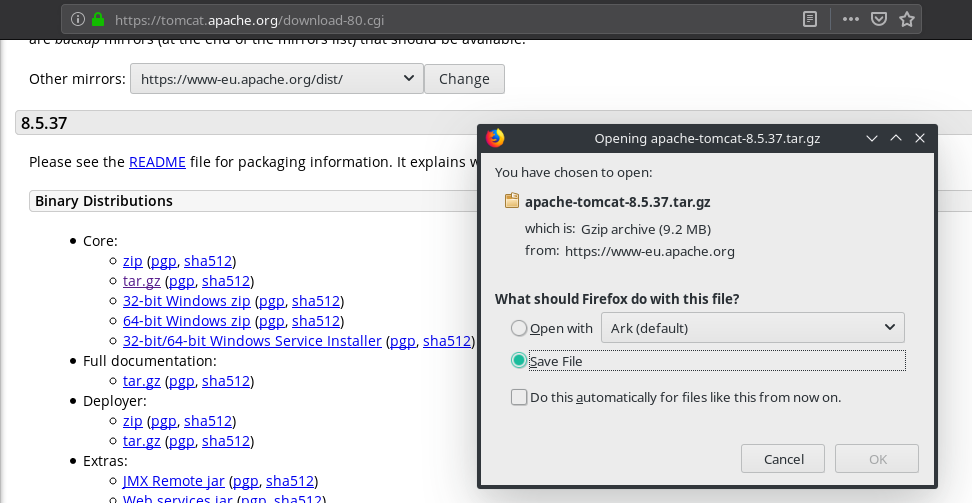
\includegraphics[width=12cm]{descarga.png}
 % estructura.png: 800x436 px, 96dpi, 21.16x11.53 cm, bb=0 0 600 327
 \caption{Se descarga el archivo comprimido de apache tomcat}
 \label{fig:descarga}
\end{center}
\end{figure}

Ahora, se puede trabajar con Tomcat desde cualquier parte pero en este caso se 
cambiara el directorio donde se va a utilizar.

Movemos el archivo .tar.gz al directorio /usr/local, lo descomprimimos y 
cambiamos el nombre de la carpeta

\begin{figure}[H]
\begin{center}
 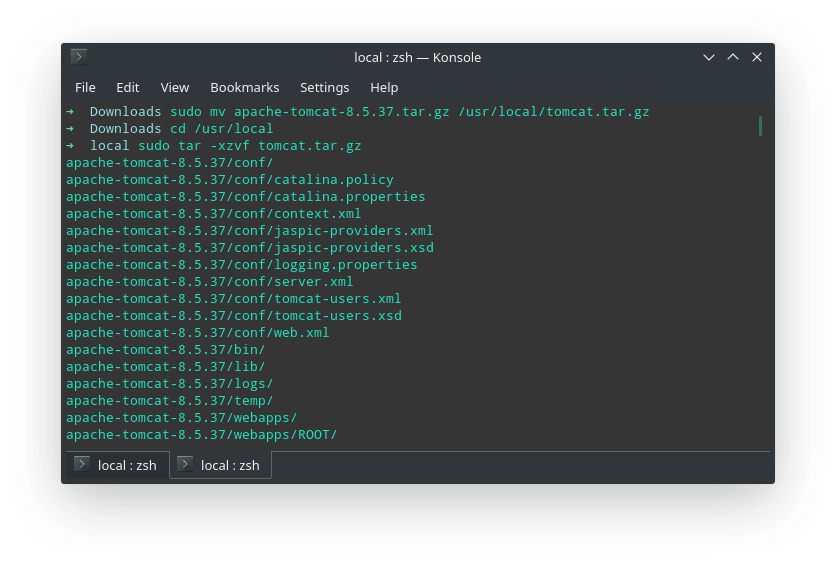
\includegraphics[width=12cm]{mover.png}
 % estructura.png: 800x436 px, 96dpi, 21.16x11.53 cm, bb=0 0 600 327
 \caption{Se descomprime el archivo}
 \label{fig:descomprimido}
\end{center}
\end{figure}

Ahora, le cambiamos el nombre de la carpeta para facilidad y para poder 
ejecutar los scripts que se encuentran dentro de de la carpeta se cambian los 
permisos de los archivos.

\begin{figure}[H]
\begin{center}
 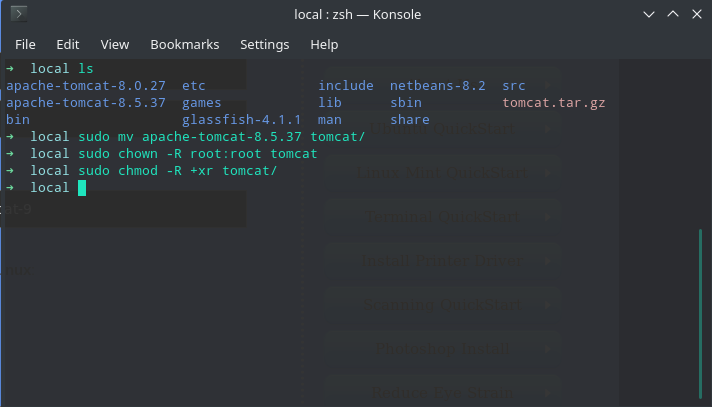
\includegraphics[width=12cm]{permisos.png}
 % estructura.png: 800x436 px, 96dpi, 21.16x11.53 cm, bb=0 0 600 327
 \caption{Cambio del nombre de carpeta y permisos}
 \label{fig:permisos}
\end{center}
\end{figure}

Finalmente, iniciamos el servidor y vamos a la pagina de inicio de Apache 
Tomcat en localhost:8080 y vemos que funciona correctamente.

\begin{figure}[H]
\begin{center}
 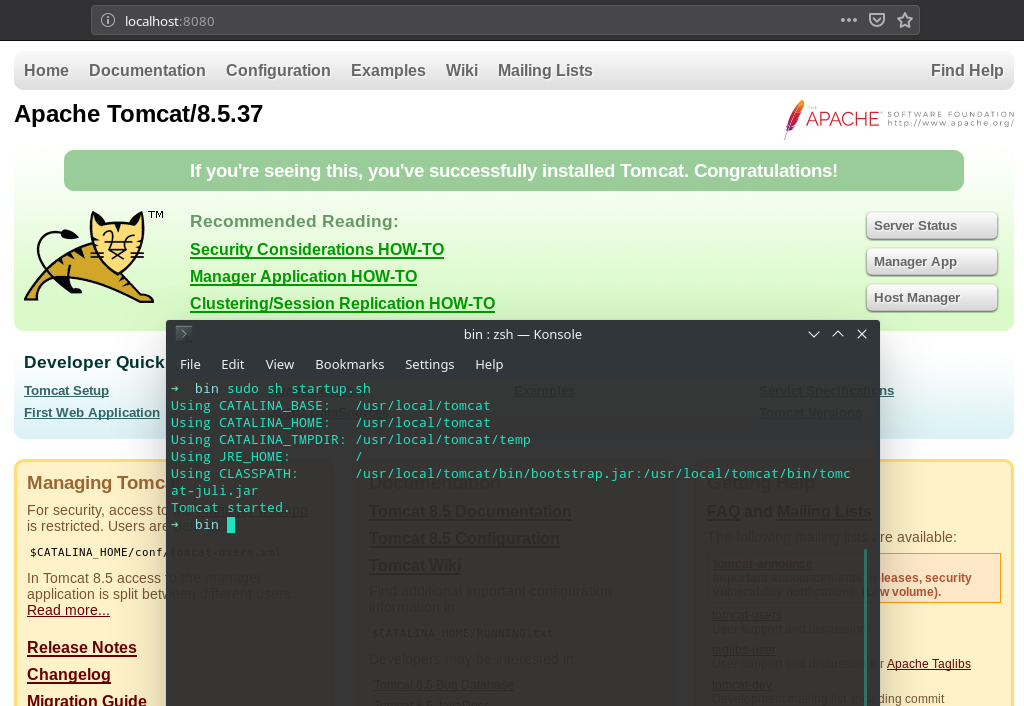
\includegraphics[width=12cm]{final.png}
 % estructura.png: 800x436 px, 96dpi, 21.16x11.53 cm, bb=0 0 600 327
 \caption{Todo funciona bien}
 \label{fig:final}
\end{center}
\end{figure}

\section{Conclusiones}
La instalación de Apache Tomcat es bastante sencilla por lo que el utilizar 
esta herramienta es una buena alternativa si se empieza a aprender el como 
desarrollar aplicaciónes web con Java EE.

\end{document}
